%=====================导=======言==============================
\documentclass[a4paper,11pt]{article}
%======================Include Packages========================

\usepackage[175]{MCMthesis}  %队号在这里填写
%\usepackage[175,nosheet]{MCMthesis}%这个参数形式可去掉summary sheet首页。
\problem{A}  %选题
%===============设置正文和数学字体=============================
%有些字体需要安装一些字体文件,注意辨别。
%我参照 MCM论文集的字体 使用如下宏包来定制字体。
\usepackage{palatino}

%设置段落之间的距离,若不需要删除或者注释掉即可。
\setlength\parskip{.5\baselineskip}

%\def\abstractname{Summary}%可修改摘要名称

%%%%%%%%%%%%%%%%%%%%%%%%%%%%%%%%%%%%%%%%%%%%%%%%%%%%%%%%%%%%%%%%%%%
%%%%%%%%%%%%%%%%%%$$$$$$$==正文开始==$$$$$$$%%%%%%%%%%%%%%%%%%%%%%%
%%%%%%%%%%%%%%%%%%%%%%%%%%%%%%%%%%%%%%%%%%%%%%%%%%%%%%%%%%%%%%%%%%%

%==========================论文标题===============================
\title{The \LaTeX Template for  MCM}
\author{\small {Maoyin Sun, Hailong Qian, Ge Jin}} 
\date{\today}
%=================================================================
%==================================================================
\begin{document}
%摘要需要放在maketitle之前才能保证运行正常
%====================摘=======要===================================
\begin{abstract}
We determine the sweet spot on a baseball bat. We capture the essential
physics of the ball–bat impact by taking the ball to be a lossy spring and the
bat to be an Euler-Bernoulli beam. To impart some intuition about the model,
we begin by presenting a rigid-body model. Next, we use our full model
to reconcile various correct and incorrect claims about the sweet spot found
in the literature. Finally, we discuss the sweet spot and the performances of
corked and aluminum bats, with a particular emphasis on hoop modes.
\begin{keywords}
keyword1; keyword2
\end{keywords}
\end{abstract}

\maketitle
\pagestyle{empty}
%
\newpage                                                          %
%==================================================================


%====================生=成=目=录===================================
%\tableofcontents                                                  %                                            %
%\newpage
\pagestyle{fancy}                                                     %
%==================================================================
\section{Introduction}
\subsection{Introduction to the Problem}
With the rapid development of science and technology, optimizing traffic flow has become an urgent demand of people around the world. Under the new conditions and prerequisites, the old rules may no longer apply. In order to address the problem above we conclude two sub-problems to tackle in our paper: 
\begin{itemize}
\item Analyze whether keep-right-except-to-pass rule work in new conditions including heavy traffic, more lanes, etc. Compare keep-right-except-to-pass rule and other alternatives and decide which is better at what need. Analyze robustness. 
\item Research how will the conclusion vary providing vehicles are controled by intellegent system. 
\end{itemize}
\subsection{Background}
Attempts to produce a mathematical theory of traffic flow date back to the 1920s, when Frank Knight first produced an analysis of traffic equilibrium, which was refined into Wardrop's first and second principles of equilibrium in 1952\cite{trafficflowhistory}. In 1950s, CA(cellular automaton) model are raised by Von Neumann, and it called much attention in 1970s. S.Wolfram first implemented this model on addressing traffic flow\cite{1983RvMP...55..601W}. Since then quantities of CA models are proposed in the realm of traffic flow theory, such as NaSch model, FI model, BML model, etc. As civilization developed, old models are more and more limited. 

\subsection{Simulation Model}
We developed a new traffic flow simulation model toolkit based on HTML5. With the function of collision pre-detection and fundamental diagram paiting, we can easily analyze the performance of individual strategies. 
\begin{figure}[H]
  \centering
  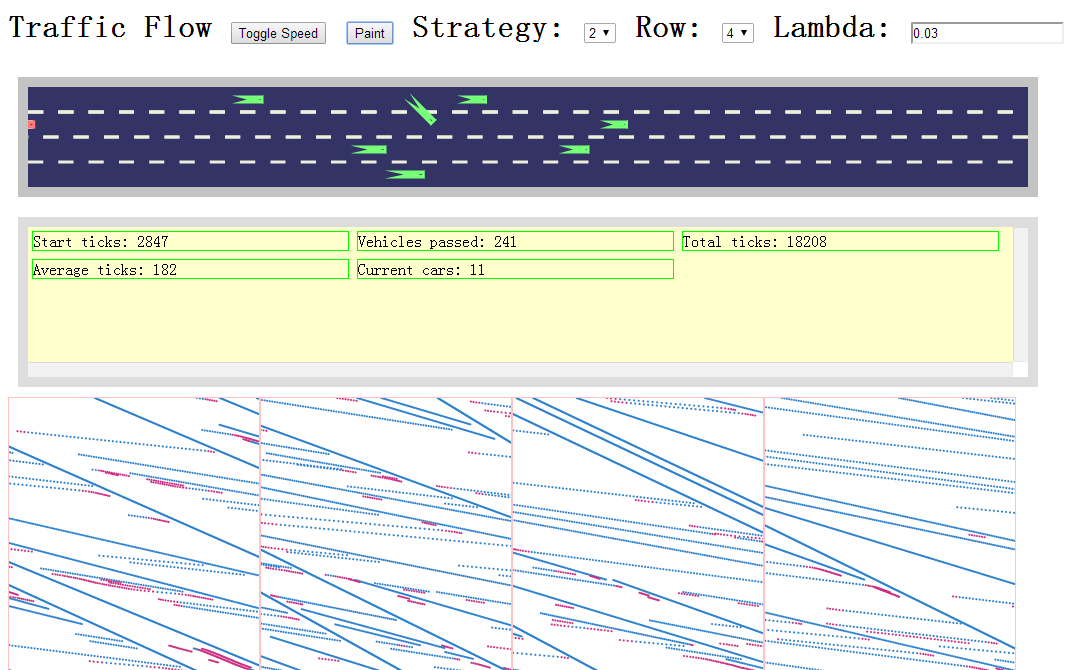
\includegraphics[width=.6\textwidth]{./img/simulationmodel.png}
  \caption{Strategy, max rows, and car amount can be changed instantly. In the fundamental diagram, blue points mean the vehicle is running at its fastest speed, red points means it's obstructed. }
  \label{fig:simulationmodel}
\end{figure}
Figure \ref{fig:simulationmodel} shows the interface simulation toolkit. And if we need faster calculation, we can toggle the animation and process with no delay. Time inside this system is based on ticks as a unit of time rather than real time, so the programme can maximize the computer capacity. 

Under this model we analyzed the formal individual strategies of vehicle drivers, estimated a trival upper bound of traffic efficiency, and tried to design an optimal self-adapting solution capable of all condition that make efficiency approach to the upper bound. 

% event loop, collision pre-detection, lane changing are expandable

\section{Assumptions}
The argumentation in this paper is based on assumptions below. 
\begin{itemize}
  \item Safety has the unconditional priority to any other goals; 
  \item Roads in this paper refer to streight equal width roads. Vehicles travls along and across equal width lanes freely; 
  \item The amount of vehicles at each time fits Poisson distribution\cite{breiman1963}; 
  \item The length, max speed of vehicles evenly distributed in specific intervals; 
  \item As both speed and accelleration are related to the performance of the vehicle, we assumpt acelleration is linear to speed; 
  \item Traveling across lanes make a car engaging two lanes for a while, and requires no other costs. 
  \item Accidents are out of account; 
  \item Other enviromental condition remain stable; 
\end{itemize}
\section{Nomenclature and Terminology}
\begin{table}[H]
  \center{
    \begin{tabular}{ccc}
      \toprule
      Variable & Description\\
      \midrule
      $R_m$ & Max width of the road, Counting by row from $0$. \\
      $\theta_f$ & Front warning ratio, impact the collision pre-detect. \\
      $\theta_b$ & Front warning ratio, impact the collision pre-detect. \\
      $a_-$ & Accelerate factor of increasing speed. \\
      $a_+$ & Accelerate factor of decreasing speed. \\
      $\lambda_p$ & Vehicles quantity factor. \\
      $\tilde{V}$ & Number of total vehicles passed by. \\
      $V^k$ & The vehicle with id $k$. \\
      $V^k_x$ & Distance the vehicle $V$ has traveled. \\
      $V^k_c$ & Speed of the vehivle $V$. \\
      $V^k_{c_{max}}$ & Max speed of vehicle $V$. \\
      \bottomrule
    \end{tabular}
  }
\end{table}
\section{Analysis}
\subsection{The Distribution of Vehicles}

\subsection{The Keep-Right-Except-To-Pass Rule}

\subsection{A Trival Upper Bound of Traffic Efficiency}

\subsection{The Difference Between Human Judgment and Intelligent System}
\paragraph{Microscopic versus Marcoscopic}
\paragraph{Individualistic versus Collectivistic}
\paragraph{More Kinetic}

\section{Model \uppercase\expandafter{\romannumeral1}: Individual Strategy Under Certain Rules}
\subsection{Existent Strategy}
Precondition: Safety First. There shall be no collision
\paragraph{The Wait-only Strategy}
\paragraph{The Keep-Right-Except-To-Pass Strategy}
\paragraph{The Speed Classifying Strategy}
\paragraph{the Dodging Rule}
\subsection{Distinctive Strategy}

\subsection{Effeciency Analysis}

\section{Model \uppercase\expandafter{\romannumeral2}: }
... 

\section{Evaluate of the Models}
\subsection{Strengths}

\subsection{Weaknesses}

\subsection{Sensitivity and Robustness}
\section{Conclusion}


\begin{thebibliography}{99}
\end{thebibliography}
%====================��¼����������==========================================
\begin{appendices}
%\renewcommand{\thesection}{\Alph{chapter}.}
\section{First appendix}
Here are simulation programmes we used in our model as follow.\\
\textbf{\textcolor[rgb]{0.98,0.00,0.00}{Input matlab source:}}
\lstinputlisting[language=Matlab]{./code/matlab1.m}
\section{Second appendix}
some more text\textcolor[rgb]{0.98,0.00,0.00}{\textbf{Input C++ source:}}
\lstinputlisting[language=C++]{./code/sudoku.cpp}
\end{appendices}



\end{document}
%%%%%%%%%%%%%%%%%%%%%%%%%%%%%%%%%%%%%%%%%%%%%%%%%%%%%%%%%%%%%%%%%%%
%%%%%%%%%%===========THE END OF PAPER============%%%%%%%%%%%%%%%%%%
%%%%%%%%%%%%%%%%%%%%%%%%%%%%%%%%%%%%%%%%%%%%%%%%%%%%%%%%%%%%%%%%%%%
